% cxy批注修改：按投稿清晰度要求适当放大密集图，使主要标注接近图题字号；原矢量内容与数据不变。
% Compile manuscript_english.tex.
% 中文备注：单栏直接置于分解覆盖范围说明段后，避免浮动到图4之后。
\begin{figure}[!htbp]\centering
\makeatletter\def\@captype{figure}\makeatother
\par
% 本轮修改：三幅示意图采用矢量重绘，按单栏重排，坐标和子图标签清晰。
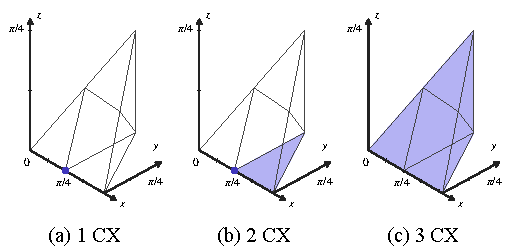
\includegraphics[width=\linewidth]{assets/fig03_cx_gate_coverage_revised.pdf}
\par

\vspace{2pt}
\caption{Regions accessible with different numbers of CX gates.}\label{fig:3}
% 翻译：图3：由多个CX门生成的局部等价类区域。
\end{figure}
